% ==================================================
% CHAPTER 2: Characterization of sTGCs using cosmic rays %
% ==================================================

\chapter{Characterization of sTGCs using cosmic rays}
\label{chap:cosmics}
% Edit count: Lia - 0, Brigitte - 0

In Canada, the cathode boards were prepared at TRIUMF in Vancouver, British Columbia; the quadruplets were constructed at Carleton University in Ottawa, Ontario; and were tested and characterized with cosmic muons at McGill University in Montreal, Quebec. Cosmic muon characterization was done with a typical hodoscope.  The quadruplet was placed in the test bench (of which a complete description can be found in Lefebvre, 2018~\cite{lefebvre_thesis}). Above and below it was a layer of scintillator-PMT arrays, labelled in figure~\ref{fig:hodoscope}. If one scintillator from each array fired in coincidence, it indicated the passage of a cosmic muon to be recorded by the quadruplet. The trigger was passed \iffalse through a KC705\footnote{Xilinx, Xilinx Kintex-7 FPGA KC705 Evaluation Kit, EK-K7-KC705-G, 2018} which sent it \fi to the front end boards (FEBs) attached to the adaptor boards of each layer of the quadruplet to readout the electrodes.

\section{Collecting cosmic muon data}
\begin{figure}
    \centering
    \includegraphics[width = 0.9\textwidth]{figures/figure_test_bench.png}
    \caption{Cosmic muon hodoscope at McGill University with sTGC quadruplet in position.}
    \label{fig:hodoscope}
\end{figure}

% It would be great to have a scope trace here, preferably of a strip. Oops.
Each sTGC electrode was connected to a channel on an ASIC\footnote{VMM3~\cite{iakovidis_vmm3_2017}} on the FEB, which was set to measure and record the channel's maximum output (called peak detector output, or PDO) \textcolor{red}{if the channel was above threshold}. Thresholds were measured~\cite{chen_calibration_2019} and adjusted manually in the configuration/readout software (\package{stgc\_readout\_sw}~\cite{siyuan_sun_stgc_readout_sw}). For each trigger, the PDO of all channels above threshold were recorded and stored in a binary file, which could be decoded into a usable ROOT tree~\cite{ROOT} by \package{tgc\_analysis/vmm3Decoder}~\cite{lefebvre_tgc_analysis}. A event recorded in the tree corresponded to one trigger of the scintillator-PMT arrays. 

%TODO : Redo this section once you're sure what figures you're using.
The package \package{tgc\_analysis/CosmicsAnalysis}~\cite{lefebvre_tgc_analysis} was used to characterize quadruplets. Many of the characterization methods were based on rebuilding muon tracks. The x and y positions of the muon track on each layer were extracted from the signal on the wires and strips respectively, as shown in figure~\ref{fig:coord_system}. The x-coordinate was taken as the center of the wire group with the maximum PDO, since the wires' pitch was larger than the typical charge spreading. The y-coordinate was taken as the Gaussian mean of the PDO distribution across groups of contiguous strips. The process of grouping contiguous strips that fired was called clustering, and the resulting group was called a cluster. A sample cluster is shown in figure~\ref{fig:sample_cluster}.

%TODO : Use fig 2.12 pg 36 Benoit's thesis on left with sample cluster on right for fig:sample_cluster and REMOVE this. Rewrite text to match figure scheme.
\begin{figure}
    \centering
    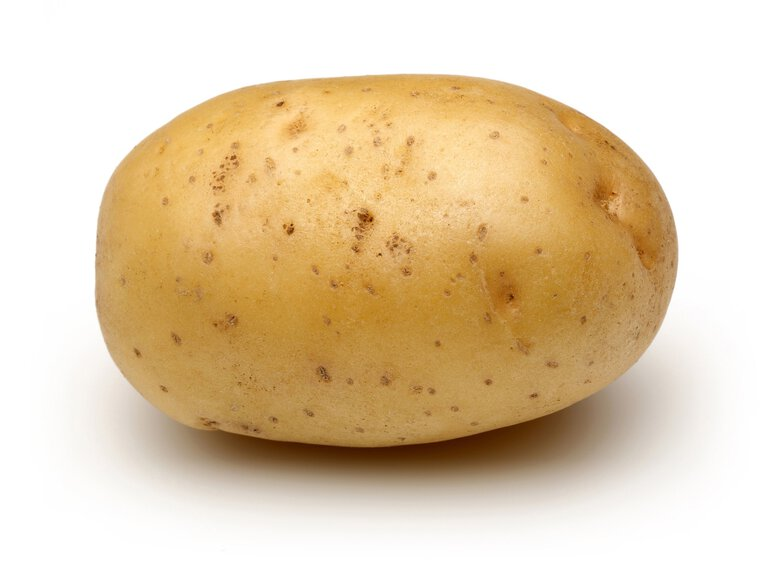
\includegraphics[width = 0.9\textwidth]{figures/potato.jpg}
    \caption{Coordinate system for the hits on each layer of an sTGC. The x-axis is perpendicular to the wires and the y-axis is perpendicular to the strips. The z-axis (not pictured) is centered between layer 2 and 3 and points towards layer 4. This is the coordinate system used in \package{tgc\_analysis}~\cite{lefebvre_tgc_analysis}.}
    \label{fig:coord_system}
\end{figure}

\begin{figure}
    \centering
    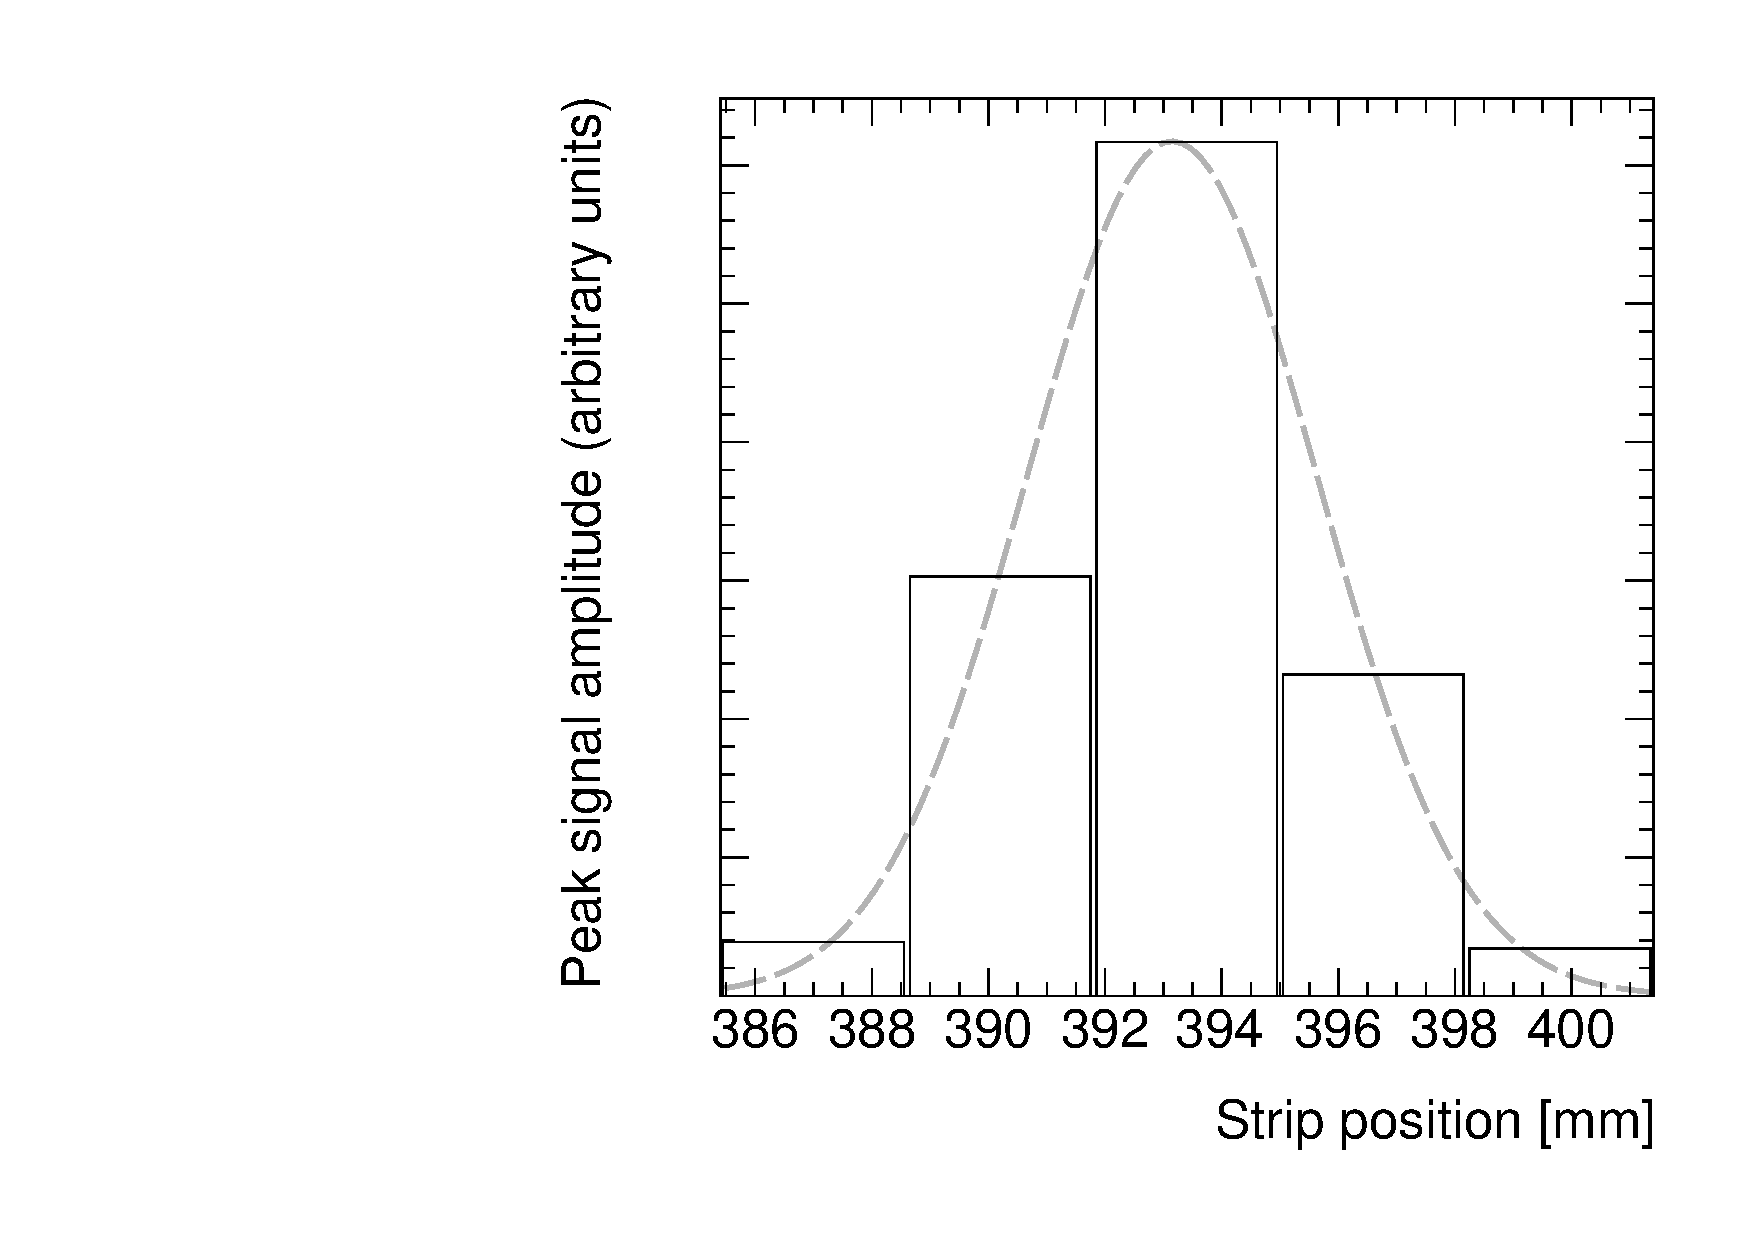
\includegraphics[width = 0.9\textwidth]{figures/sample_cluster_QL2C04_event5_layer2.pdf}
    \caption{A sample cluster resulting from the current picked up on a group of strips (presumably) after the passing of a muon. The grey line is a Gaussian fit.}
    \label{fig:sample_cluster}
\end{figure}

Note that for strips, the hardware was configured to also record the PDO of strips adjacent to a strip above threshold during cosmic muon testing.

After the coordinates of the muon's passage were estimated on all layers, tracks were reconstructed in x and y separately as a step towards characterization metrics like electrode efficiency and spatial resolution~\cite{lefebvre_thesis}. 

The uncertainty in the cluster mean could be taken as the fitted mean's statistical uncertainty; however, after comparing the difference in cluster means for different fitting algorithms in appendix~\ref{sec:appendix_clustering_cluster_fit}, \SI{60}{\micro\meter} of uncertainty was assigned to the cluster means for the work in this thesis.
    
%TODO : Mention slow control and gas system where?
%TODO : Mention 2900V vs 3100V where?
%TODO : Mention uncertainty on hit x-position where?
%TODO : Does Tony do Twiki hits map?